% !TEX root = ../main.tex
% SECTION 4: GLEICHSTROMKREISE
% ============================================================

\StartChapter{Gleichstromkreise}

\begin{runintext}
Formeln zu Strömen und Spannungen in Gleichstromschaltungen: Definition von \ZSFkeyword*{Strom} und \ZSFkeyword*{Stromdichte}, \ZSFkeyword*{Ohm'sches Gesetz}, Widerstände, Leistung, reale Spannungsquellen, \ZSFkeyword*{Kirchhoff-Regeln}, Ersatzwiderstände und \ZSFkeyword*{RC-Zeitkonstanten}. Nützlich bei allen Aufgaben zu einfachen und zusammengesetzten Gleichstromkreisen, Messgeräten und Ent- bzw.\ Aufladung von Kondensatoren.
\end{runintext}

\SubsectionBar[sec:current-drift]{Strom, Drift}
\ZSFindex{Strom}
\ZSFindex{Stromdichte}
\begin{runintext}
Zusammenhänge zwischen \ZSFkeyword*{mikroskopischer Ladungsbewegung} und makroskopischem \ZSFkeyword*{Strom}; elektrischer Strom ist die Rate des \ZSFkeyword*{Ladungsflusses} durch eine Querschnittsfläche $A$.
\end{runintext}
\begin{formulabox}
\[ I = \frac{\Delta q}{\Delta t} \quad \text{mit } q = N e \quad\Rightarrow\quad \frac{\Delta N}{\Delta t} = \frac{I}{e} \]
\formulanote{Definition Strom ($[I] = \si{A} = \si{C/s}$) \& Teilchenrate ($N$: Teilchenzahl, $e$: \ZSFkeyword*{Elementarladung}).}
\formulasep
\[ I = n\,q\,A\,v_{\mathrm{d}} \qquad \vec{\jmath} = n\,q\,\vec{v}_{\mathrm{d}} \quad (q = -e \text{ für Elektronen}) \]
\formulanote{Mikroskopisch: $n = N/V$ (\ZSFkeyword{Ladungsträgerdichte} in $[\si{m^{-3}}]$), $v_{\mathrm{d}}$: \ZSFkeyword{Driftgeschwindigkeit}.}
\formulasep
\[ j = \frac{I}{A} \quad ([\vec{\jmath}] = \si{A/m^2}) \qquad I = \iint_A \vec{\jmath} \cdot \mathrm{d}\vec{A} \]
\formulanote{Makroskopische \ZSFkeyword{Stromdichte} $\vec{\jmath}$. Strom $I$ ist Fluss von $\vec{\jmath}$ durch Fläche $A$.}
\end{formulabox}

\SubsectionBar[sec:ohms-law]{Ohm}
\ZSFindex[Leitfahigkeit]{Leitfähigkeit}
\ZSFindex{Widerstand}
\ZSFindex{Spezifischer Widerstand}
\ZSFindexsee{Ohm}{Widerstand}
\ZSFindexsee{Gesetz von Ohm}{Ohm'sches Gesetz}
\ZSFindex{Temperaturkoeffizient}
\begin{runintext}
Das \ZSFkeyword[Ohm'sches Gesetz]{Ohm'sche Gesetz} und die Berechnung von Widerständen aus Materialeigenschaften; zentral für die Analyse von Stromkreisen.
\end{runintext}
\begin{formulabox}
\[ R = \frac{U}{I} \quad \text{($[R] = \Omega = \text{V/A}$)} \]
\[ U = R\,I \quad \text{($R$ konstant)} \]
\formulanote{Zweck: Definition des elektrischen Widerstands und makroskopisches Ohm'sches Gesetz.}
\end{formulabox}

\begin{formulabox}
\[ R = \rho\,\frac{\ell}{A} \quad \text{spezifischer Widerstand $\rho$ in $[\Omega\cdot\text{m}]$} \]
\formulanote{Zweck: Berechnung des Widerstands aus Geometrie ($\ell, A$) und Material ($\rho$). $\ell$ ist die Länge entlang des \ZSFkeyword{Strompfads}, $A$ der Querschnitt senkrecht dazu — Form und Krümmung des Leiters ändern $R$ nicht. \ZSFdanger{Achtung:} nur bei eindeutigem Strompfad; bei mehreren Wegen zwischen denselben Kontakten (Ring, Rohr, Schichtleiter) zuerst in Teilstücke zerlegen und kombinieren \ZSFref{sec:equivalent-resistance}.}
\end{formulabox}

\begin{formulabox}
\[ \alpha = \frac{(\rho-\rho_0)/\rho_0}{T-T_0} \quad \text{Temperaturkoeffizient} \]
\[ \rho = \rho_0\,\bigl(1 + \alpha(T-T_0)\bigr) \]
\formulanote{Zweck: Temperaturabhängigkeit des spezifischen Widerstands.}
\end{formulabox}

\begin{formulabox}
\[ \vec{E} = \rho\,\vec{\jmath} = \frac{\vec{\jmath}}{\sigma} \quad \text{lokales Ohm'sches Gesetz} \]
\formulanote{Zweck: Lokales Ohm'sches Gesetz (Zusammenhang zwischen elektrischem Feld und Stromdichte).}
\end{formulabox}
\begin{runintext}
$\ell$: Länge, $A$: Querschnitt, $\rho$: spez.\ Widerstand, $\sigma$: Leitfähigkeit ($1/\rho$), $\alpha$: Temp.-Koeff., $T_0$: Bezugstemp.\ (meist $20^\circ\text{C}$).
\end{runintext}

\SubsectionBar[sec:electric-power]{Leistung}
\ZSFindexsee{Watt}{Leistung}
\ZSFindex{Spannungsquelle}
\begin{runintext}
Berechnung von \ZSFkeyword[Leistung]{elektrischer Leistung} und umgesetzter Energie; grundlegend für Leistungsbilanzen und Erwärmung von Bauteilen.
\end{runintext}
\begin{formulabox}
\[ P = \frac{\mathrm{d}E}{\mathrm{d}t} \quad \text{allgemeine Definition} \]
\[ P = I\,U \quad \text{Bauelement} \]
\formulasep
\[ P = I\,U_R = R\,I^2 = \frac{U^2}{R} \quad \text{am Widerstand} \]
\formulasep
\[ P = I\,U_Q \quad \text{Spannungsquelle} \]
\[ E_{\mathrm{el}} = q\,U_Q \quad \text{gespeicherte Energie Batterie} \]
\formulanote{Zweck: Elektrische Leistung (allgemein, am Widerstand, an Quelle mit Quell-/Leerlaufspannung $U_Q$); gespeicherte Energie. Quercheck: $\sum P_{\mathrm{Quelle}} = \sum P_{\mathrm{Widerstand}}$ (Leistungserhaltung).}
\end{formulabox}

\begin{minipage}{\linewidth}
\SubsectionBar[sec:kirchhoff-current]{Knotenregel}
\ZSFindex{Knotenregel}
\ZSFindex{Kirchhoff-Regeln}
\ZSFindexsee{Regeln von Kirchhoff}{Kirchhoff-Regeln}
\begin{runintext}
Summe der zufliessenden Ströme ist gleich der Summe der abfliessenden Ströme an einer \ZSFkeyword*{Verzweigung}.
\end{runintext}
\begin{defbox}[Knotenregel]
\begin{splitbox}[0.4]
    \centering
    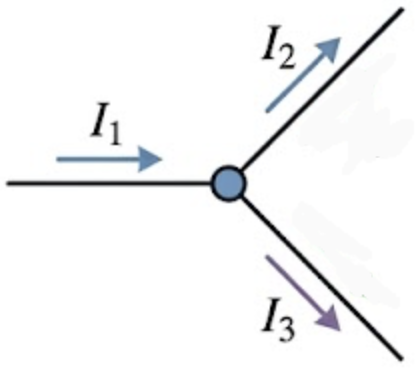
\includegraphics[width=\linewidth, keepaspectratio]{graphics/knotenregel.png}
    \tcblower
    \begin{formulabox}
        \[ \sum I_{\mathrm{zu}} = \sum I_{\mathrm{ab}} \]
    \end{formulabox}
\end{splitbox}
\formulanote{Strom $I_1$ teilt sich in $I_2$ und $I_3$ auf. \textbf{Zweck:} Strombilanz an Knotenpunkten im Netzwerk.}
\end{defbox}
\end{minipage}

\begin{minipage}{\linewidth}
\SubsectionBar[sec:kirchhoff-voltage]{Maschenregel}
\ZSFindex{Innenwiderstand}
\ZSFindex{Klemmenspannung}
\ZSFindex{Spannungsquelle}
\begin{runintext}
Die Summe aller Spannungsabfälle in einer geschlossenen Schleife (\ZSFkeyword[Maschenregel]{Masche}) ist null.
\end{runintext}
\begin{defbox}[Maschenregel]
\begin{splitbox}[0.4]
    \centering
    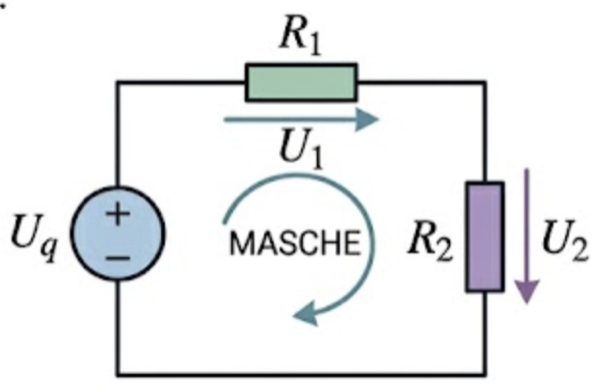
\includegraphics[width=\linewidth, keepaspectratio]{graphics/maschenregel.png}
    \tcblower
    \begin{formulabox}
        \[ \sum U_k = 0 \]
        \formulasep
        \[ \varphi_a - \varphi_b = U_Q - R_{\mathrm{in}}\,I \]
    \end{formulabox}
\end{splitbox}
\formulanote{Summe aller Spannungen in geschlossener Schleife ist $0$. Masche: Spannungsabfall in Stromrichtung ist negativ. Reale Batterie: Klemmenspannung bei Innenwiderstand.}
\end{defbox}
\end{minipage}

\SubsectionBar[sec:equivalent-resistance]{Ersatzwiderstände}
\ZSFindex{Ersatzwiderstand}
\begin{runintext}
Regeln zur Kombination von \ZSFkeyword[Reihenschaltung / Serienschaltung]{in Reihe} und \ZSFkeyword[Parallelschaltung]{parallel} geschalteten Widerständen zur einfachen Reduktion von Teilschaltungen.
\end{runintext}
\begin{formulabox}
\[ R = R_1 + R_2 + R_3 + \cdots \quad \text{Reihe} \]
\formulasep
\[ \frac{1}{R} = \frac{1}{R_1} + \frac{1}{R_2} + \frac{1}{R_3} + \cdots \quad \text{Parallel} \]
\[ R = \frac{R_1 R_2}{R_1 + R_2} \quad \text{2 Stück parallel} \]
\formulanote{Zweck: Ersatzwiderstand Reihen- bzw.\ Parallelschaltung.}
\end{formulabox}

\SubsectionBar[sec:rc-circuits]{RC-Kreise}
\ZSFindex{RC-Kreis / RC-Zeitkonstante}
\ZSFindex{Zeitkonstante}
\begin{runintext}
Zeitabhängiges Verhalten von Strom und Ladung beim \ZSFkeyword[Aufladung]{Auf-} und \ZSFkeyword[Entladung]{Entladen} von Kondensatoren über Widerstände.
\end{runintext}
\begin{runintext}
\ZSFkeyword{Amperemeter}: kleiner $R$, in Reihe. \ZSFkeyword{Voltmeter}: grosser $R$, parallel. \ZSFkeyword{Ohmmeter}: Batterie + Galvanometer + $R$.
\end{runintext}
\begin{formulabox}
\[ q(t) = q_0\,\mathrm{e}^{-t/(RC)} = q_0\,\mathrm{e}^{-t/\tau} \quad \text{Entladung} \]
\[ I(t) = -\frac{\mathrm{d}q}{\mathrm{d}t} = \frac{U_{C,0}}{R}\,\mathrm{e}^{-t/\tau} = I_0\,\mathrm{e}^{-t/\tau} \]
\formulanote{Zweck: Zeitlicher Verlauf von Ladung $q(t)$ und Entladestrom $I(t)$ beim Entladen eines Kondensators.}
\end{formulabox}

\begin{formulabox}
\[ \tau = R\,C \quad \text{Zeitkonstante} \]
\formulanote{Zweck: Definition der RC-Zeitkonstante $\tau$ (Zeit, nach der Ladung/Strom auf $1/\mathrm{e} \approx 37\%$ abgefallen bzw. Ladung auf $1 - 1/\mathrm{e} \approx 63\%$ angestiegen ist).}
\end{formulabox}

\begin{formulabox}
\[ q(t) = C\,U\,(1 - \mathrm{e}^{-t/\tau}) = q_E\,(1 - \mathrm{e}^{-t/\tau}) \quad \text{Aufladung} \]
\[ I(t) = \frac{U}{R}\,\mathrm{e}^{-t/\tau} = I_0\,\mathrm{e}^{-t/\tau} \]
\formulanote{$q_E = C\,U$ (max.\ Ladung). \ZSFdanger{Achtung:} $U$ ist die konstante Quellspannung (Batterie), NICHT die veränderliche Kondensatorspannung $U_C(t) = q(t)/C$.}
\end{formulabox}

\begin{propertylist}[Grenzverhalten (Schaltmomente)]
    \ZSFFact{Direkt nach Schalten ($t=0$)}{Ungeladener Kondensator wirkt wie \ZSFkeyword{Kurzschluss} ($U_C = 0$, maximaler Strom $I_0 = U/R$).}
    \ZSFFact{Nach langer Zeit ($t\to\infty$)}{Geladener Kondensator wirkt wie \ZSFkeyword*{Leitungsunterbrechung} (Strom $I \to 0$, $U_C \to U$).}
\end{propertylist}

% ============================================================

\ZSFfig{graphics/Kondensator_Lade_und_Entladekurve_Spannung_Strom.png}{Lade-/Entladekurve (RC)}{Exponentialverlauf $U_C(t)$ und $I(t)$ mit $\tau=RC$}
